When we first deployed ORES, we reached out to several different wiki communities and invited them to test the system for use in patrolling for vandalism.  In these announcements, we encouraged editors to install ScoredRevisions, the only tool that used ORES's edit quality models at the time.  ScoredRevisions both highlights edits that are likely to be damaging (as predicted by the model) and displays the likelihood of the prediction as a percentage.

Before long, our users began filing false-positive reports on wiki pages of their own design---some after our request, but mostly on their own.  In this section, we describe three cases where our users independently developed these false-positive reporting pages and how they used them to understand ORES, the roles of automated quality control in their own spaces, and to communicate with us about model bias.

\subsection{Report mistakes (Wikidata)}
\begin{figure}[h]
  \centering
  \includegraphics[width=.45\textwidth]{figures/ORES_report_mistakes_table}
  \caption{A slice of the ORES report mistakes table in Wikidata.}
  \label{fig:ores_report_mistakes}
\end{figure}

When we first deployed prediction models for Wikidata---a free and open knowledge base that can be read and edited by both humans and machines\footnote{\url{https://wikidata.org}}---we were breaking new ground by building a damage detection classifier based on a structured data wiki\cite{sarabadani2017building}.  We created a page called ``Report mistakes'' and invited users to tell us about mistakes that the prediction model made on that page. We left the format and structure largely up to the users.

Within 20 minutes, we received our first report.  As reports streamed in, we began to respond to them and make adjustments to the model building process to address data extraction bugs and to increase the signal so that the model differentiate damage from non-damaging edits.  After a month of reports and bug fixes, we decided to build a table to represent the progress that we made in iterations on the model against the reported false-positives (Figure~\ref{fig:ores_report_mistakes}).  Each row represents false-positive, and each column describes the progress we made in not detecting those edits as damaging in subsequent iterations of the model.  Through this process, we learned how Wikidata editors understood and saw damage, as well as how our modeling and feature extraction process captured signals in ways that differed from Wikidata editors' understandings.  Because of this back-and-forth collaboration made possible through ORES's various features, we were able to publicly demonstrate improvements to this community.

\subsection{Patrolling/ORES (Italian Wikipedia)}
Italian Wikipedia was one of the first wikis where we deployed basic edit quality models.  Our local collaborator, who helped us develop the language specific features, User:Rotpunkt, created a page for ORES\footnote{\url{https://it.wikipedia.org/wiki/Progetto:Patrolling/ORES}} with a section for reporting false-positives (``falsi positivi'').  Within several hours, Rotpunkt and a few other editors noticed some trends in their false positive reports.  These editors began to collect false positives under different headers representing themes they were seeing.  Through this process, editors from Italian Wikipedia were effectively performing an inductive, grounded theory-esque exploration ORES errors, trying to identify themes and patterns in the errors that ORES was making.

One of the themes they identified fell under the header: ``corrections to the verb for \emph{have}'' (``correzioni verbo avere'').  It turns out that the word ``ha'' in Italian translates to the English verb ``to have''.  While in Engligh and many other langauges, ``ha'' is laughing and adding ``ha'' repeatedly is a common type of vandalism seen in all langauges of Wikipedia.  We'd built a common feature in the damage model called ``informal words'' that captured these types of patterns.  But in this case, it was clear that in Italian ``ha'' should not carry signal while ``hahaha'' still should.

Because of the work of Rotpunkt and his collaborators in Italian Wikipedia, we were able to recognize the source of this issue (a set of features intended to detect the use of \emph{informal language} in articles) and to remove ``ha'' from that list for Italian Wikipedia.

\subsection{PatruBOT (Spanish Wikipedia)}
Soon after we released support for Spanish Wikipedia, a volunteer developer made a bot to automatically revert damaging edits using ORES's predictions for the ``damaging'' model (PatruBOT).  This bot was not running for long before our discussion pages were bombarded with confused Spanish-speaking editors asking us questions about why ORES did not like their work.  We struggled to understand the origin of the complaints until someone reached out about PatruBOT and its activities.

When we examined the case, we found it was one of tradeoffs between precision/recall and false positives/negatives---a common issue with machine learning applications. We concluded that PatruBOT's threshold for reverting was too sensitive. ORES reports a classification and a probability score, but it is up to the developers to decide if, for example, the bot will only auto-revert edits classified as damage with a .90, .95, .99, or higher likelihood estimate. A higher threshold will minimize the chance a good edit will be mistakenly auto-reverted, but also increase the chance that a bad edit will not be auto-reverted.  Ultimately, deciding where to draw the line between false positives and false negatives is a decision for that volunteer editing community.

The Spanish Wikipedians who were concerned with these issues began a discussion about PatruBOT's activities and blocked the bot until the issue was sorted. Using wiki pages, they organized an crowdsourced evaluation of the fitness of PatruBOT's behavior\footnote{\url{https://es.wikipedia.org/wiki/Wikipedia:Mantenimiento/Revisi\%C3\%B3n_de_errores_de_PatruBOT\%2FAn\%C3\%A1lisis}}.  This evaluation and discussion is ongoing, \footnote{\url{https://es.wikipedia.org/wiki/Wikipedia:Caf\%C3\%A9\%2FArchivo\%2FMiscel\%C3\%A1nea\%2FActual\#Parada_de_PatruBOT}} but it shows how stakeholders do not need to have an advanced understanding in machine learning evaluation to meaningfully participate in a sophisticated discussion about how, when, why, and under what conditions such classifiers should be used.

\subsection{Bias against anonymous editors}
\begin{figure*}[h!]
\centering
\begin{subfigure}[t]{.33\textwidth}
  \centering
  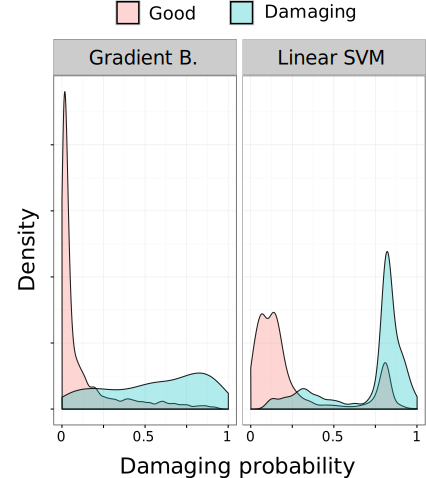
\includegraphics[width=.85\textwidth]{figures/natural_damaging_gb_vs_svc}
  \caption{No injected features}
  \label{fig:natural_damaging_gb_bs_svc}
\end{subfigure}~~
\begin{subfigure}[t]{.33\textwidth}
  \centering
  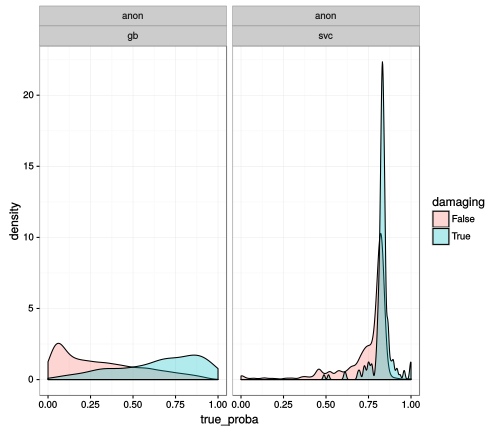
\includegraphics[width=.85\textwidth]{figures/anon_damaging_gb_vs_svc}
  \caption{Everyone is anonymous}
  \label{fig:anon_damaging_gb_bs_svc}
\end{subfigure}~~
\begin{subfigure}[t]{.33\textwidth}
  \centering
  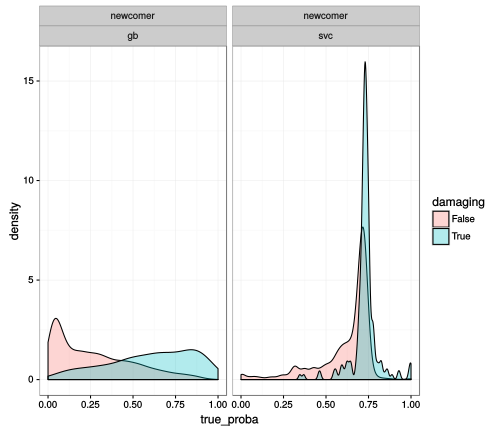
\includegraphics[width=.85\textwidth]{figures/newcomer_damaging_gb_vs_svc}
  \caption{Everyone is newly registered}
  \label{fig:newcomer_damaging_gb_bs_svc}
\end{subfigure}
\caption{The distributions of the probability of a single edit being scored as ``damaging'' based on injected features for the target user-class is presented.  Note that when injecting user-class features (anon, newcomer), all other features are held constant.}
\label{fig:prediction_error_for_anons_and_newcomers}
\end{figure*}

Shortly after we deployed ORES, we received reports that ORES's damage detection models were overly biased against anonymous editors.  At the time, we were using Linear SVM\footnote{\url{http://scikit-learn.org/stable/modules/generated/sklearn.svm.LinearSVC.html}} estimators to build classifiers, and we were considering making the transition towards ensemble strategies like GradientBoosting and RandomForest estimators.\footnote{\url{http://scikit-learn.org/stable/modules/ensemble.html}}  We took the opportunity to look for bias in the error of estimation between anonymous editors and newly registered editors.  By using our feature injection/interrogation strategy (described in Section~\ref{sec:innovations_in_openness}), we could ask our current prediction models how they would change their predictions if the exact same edit were made by a different editor.

Figure~\ref{fig:prediction_error_for_anons_and_newcomers} shows the probability density of the likelihood of ``damaging'' given three different passes over the exact same test set, using two of our modeling strategies.  Figure~\ref{fig:natural_damaging_gb_bs_svc} shows that, when we leave the features to their natural values, it appears that both models are able to differentiate effectively between damaging edits (high-damaging probability) and non-damaging edits (low-damaging probability) with the odd exception of a large amount of non-damaging edits with a relatively high-damaging probability around 0.8 in the case of the Linear SVM model.  Figures~\ref{fig:anon_damaging_gb_bs_svc} and \ref{fig:newcomer_damaging_gb_bs_svc} show a stark difference.  For the scores that go into these plots, characteristics of anonymous editors and newly registered editors were injected for all of the test edits.  We can see that the GradientBoosting model can still differentiate damage from non-damage while the Linear SVM model flags nearly all edits as damage in both case.

Through the reporting of this issue and our subsequent analysis, we were able to identify the issue and show that an improvement to our modeling strategy mitigates the problem.  Without such a tight feedback loop, we most likely would not have noticed how poorly ORES's damage detection models were performing in practice.  Worse, it might have caused vandal fighters to be increasingly (and inappropriately) skeptical of contributions by anonymous editors and newly registered editors---two groups of contributors that are already met with unnecessary hostility\footnote{\url{http://enwp.org/:en:Wikipedia:IPs_are_human_too}}\cite{halfaker2013rise}.
